% BLAST whole genome comparisons
%
% Basic BLAST/MegaBLAST whole genome comparison examples

\subsection{BLAST Whole Genome Comparisons}
% [fragile] frames must end with \end{frame} directly following a newline, or they break!
\begin{frame}[fragile]
  \frametitle{Run a megaBLAST Comparison}
  BLAST your chromosome against the comparator sequence. \\
  Put results in \texttt{chrA\_megablast\_Pba.tab}
\begin{lstlisting}[language=bash]
$ blastn -query chrA.fasta -subject NC_004547.fna -out chrA_megablast_Pba.tab -outfmt 6 
$ head -n 3 chrA_megablast_Pba.tab 
chrA	gi|50118965|ref|NC_004547.2|:10948-12453	80.34	1511	287	10	4579450	4580955	1506	1	0.0	1136
chrA	gi|50118965|ref|NC_004547.2|:c33859-32447	82.04	1409	253	0	4563151	4564559	1	1409	0.0	1201
chrA	gi|50118965|ref|NC_004547.2|:c34917-33868	82.48	1050	184	0	4562093	4563142	1	1050	0.0	 920
\end{lstlisting}
Note this defaults to using MEGABLAST...
\end{frame}
    
% [fragile] frames must end with \end{frame} directly following a newline, or they break!
\begin{frame}[fragile]
  \frametitle{Run a BLASTN Comparison}
  BLAST your chromosome against the comparator sequence \\
  Put results in \texttt{chrA\_blastn\_Pba.tab}
\begin{lstlisting}[language=bash]
$ blastn -query chrA.fasta -subject NC_004547.fna -out chrA_blastn_Pba.tab -outfmt 6 -task blastn
$ head -n 3 chrA_blastn_Pba.tab 
chrA	gi|50118965|ref|NC_004547.2|:5629-7497	79.68	1865	379	0	4584915	4586779	1865	1	0.0	1654
chrA	gi|50118965|ref|NC_004547.2|:5629-7497	92.59	27	2	0	4479367	4479393	1254	1280	0.004	41.0
chrA	gi|50118965|ref|NC_004547.2|:5629-7497	100.00	17	0	0	4613022	4613038	52	36	2.1	31.9
\end{lstlisting}
Note we added \texttt{-task blastn}
\end{frame}
    
% [fragile] frames must end with \end{frame} directly following a newline, or they break!
\begin{frame}[fragile]
  \frametitle{Do BLASTN and megaBLAST comparisons agree?}
  Check the number of alignments returned with \texttt{wc}
\begin{lstlisting}[language=bash]
$ wc chrA_megablast_Pba.tab 
    2675   32100  242539 chrA_megablast_Pba.tab
$ wc chrA_blastn_Pba.tab
   31792  381504 2850953 chrA_blastn_Pba.tab
\end{lstlisting}
  What is this telling us? \\
  Why do the results differ?
\end{frame}

\begin{frame}
  \frametitle{BLASTN vs megaBLAST}
  \begin{itemize}
    \item<1-> Legacy BLASTN uses the BLAST algorithm, megaBLAST does not
    \begin{itemize}
      \item (though BLAST+ BLASTN now uses megaBLAST by default)
    \end{itemize}      
    \item<1-> megaBLAST uses a fast, greedy algorithm due to Zhang et al. (2000) \url{http://www.ncbi.nlm.nih.gov/pubmed/10890397}
    \item<2-> megaBLAST is optimised for
    \begin{itemize}
      \item genome-level searches
      \item queries on large sequence sets (automatic query packing)
      \item long alignments of similar sequences, with SNPs/sequencing errors
    \end{itemize}
    \item<2-> A discontinuous mode (dc-megaBLAST) is recommended for more divergent sequences
  \end{itemize}
\end{frame}

\begin{frame}[fragile]
  \frametitle{Viewing alignments in ACT}
  Start ACT from the command line:
\begin{lstlisting}[language=bash]
$ act &
\end{lstlisting}
  \begin{center}
    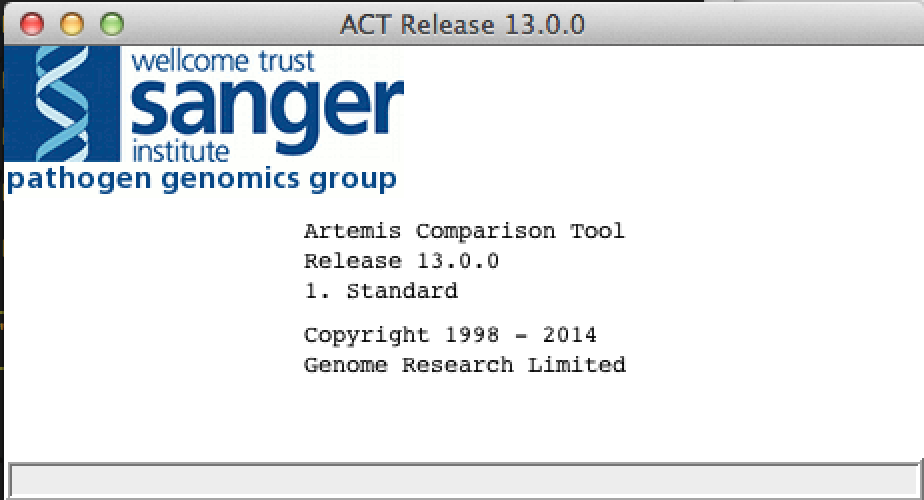
\includegraphics[width=0.6\textwidth]{images/act_wgs1}
  \end{center}
\end{frame}

\begin{frame}
  \frametitle{Use the ``File'', ``Open...'' menu item}
  \begin{center}
    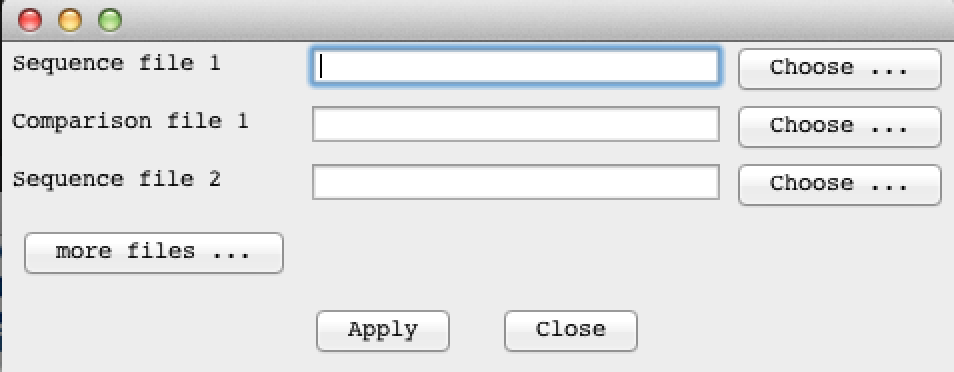
\includegraphics[width=0.9\textwidth]{images/act_wgs2}
  \end{center}
\end{frame}

\begin{frame}
  \frametitle{Increase the Number of Comparisons}
  Use \texttt{more files ...}
  \begin{center}
    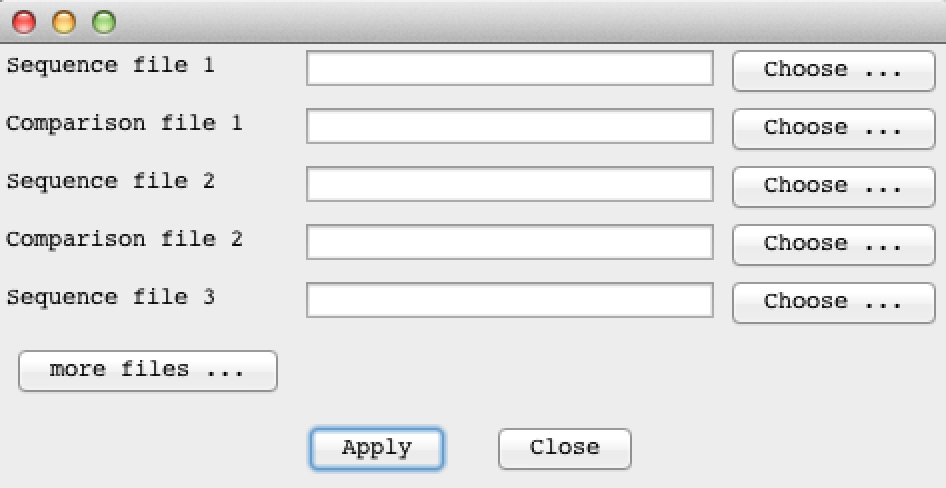
\includegraphics[width=0.9\textwidth]{images/act_wgs3}
  \end{center}
\end{frame}

\begin{frame}
  \frametitle{Select chromosome sequences}
  \begin{center}
    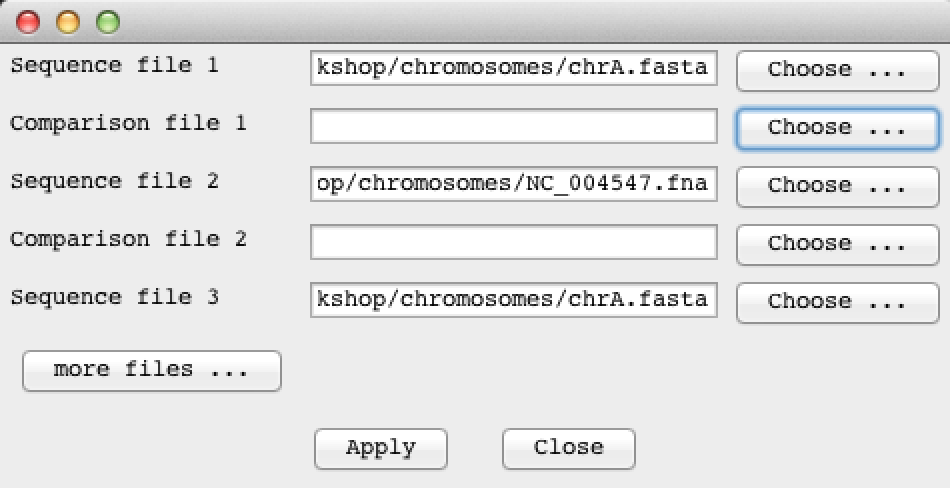
\includegraphics[width=0.9\textwidth]{images/act_wgs4}
  \end{center}
\end{frame}

\begin{frame}
  \frametitle{Add BLAST/megaBLAST results}
  \begin{center}
    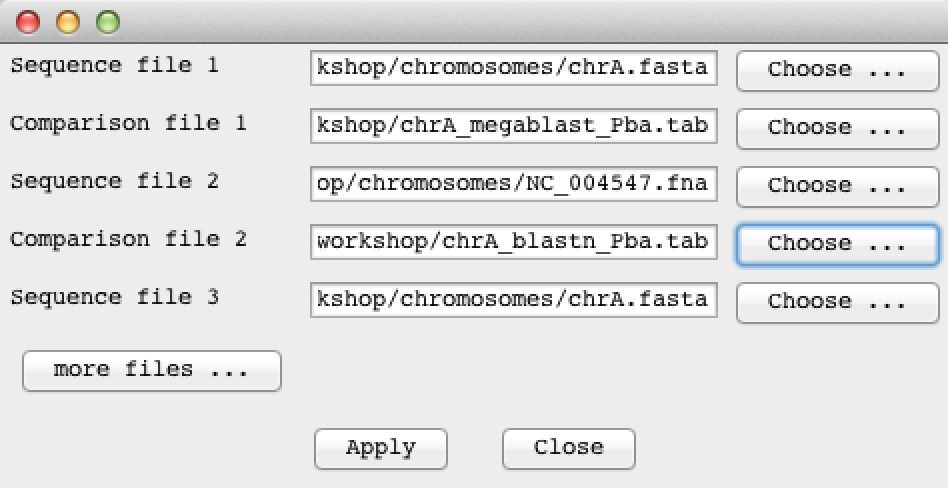
\includegraphics[width=0.9\textwidth]{images/act_wgs5}
  \end{center}
\end{frame}

\begin{frame}
  \frametitle{Zoom Out}
  \begin{center}
    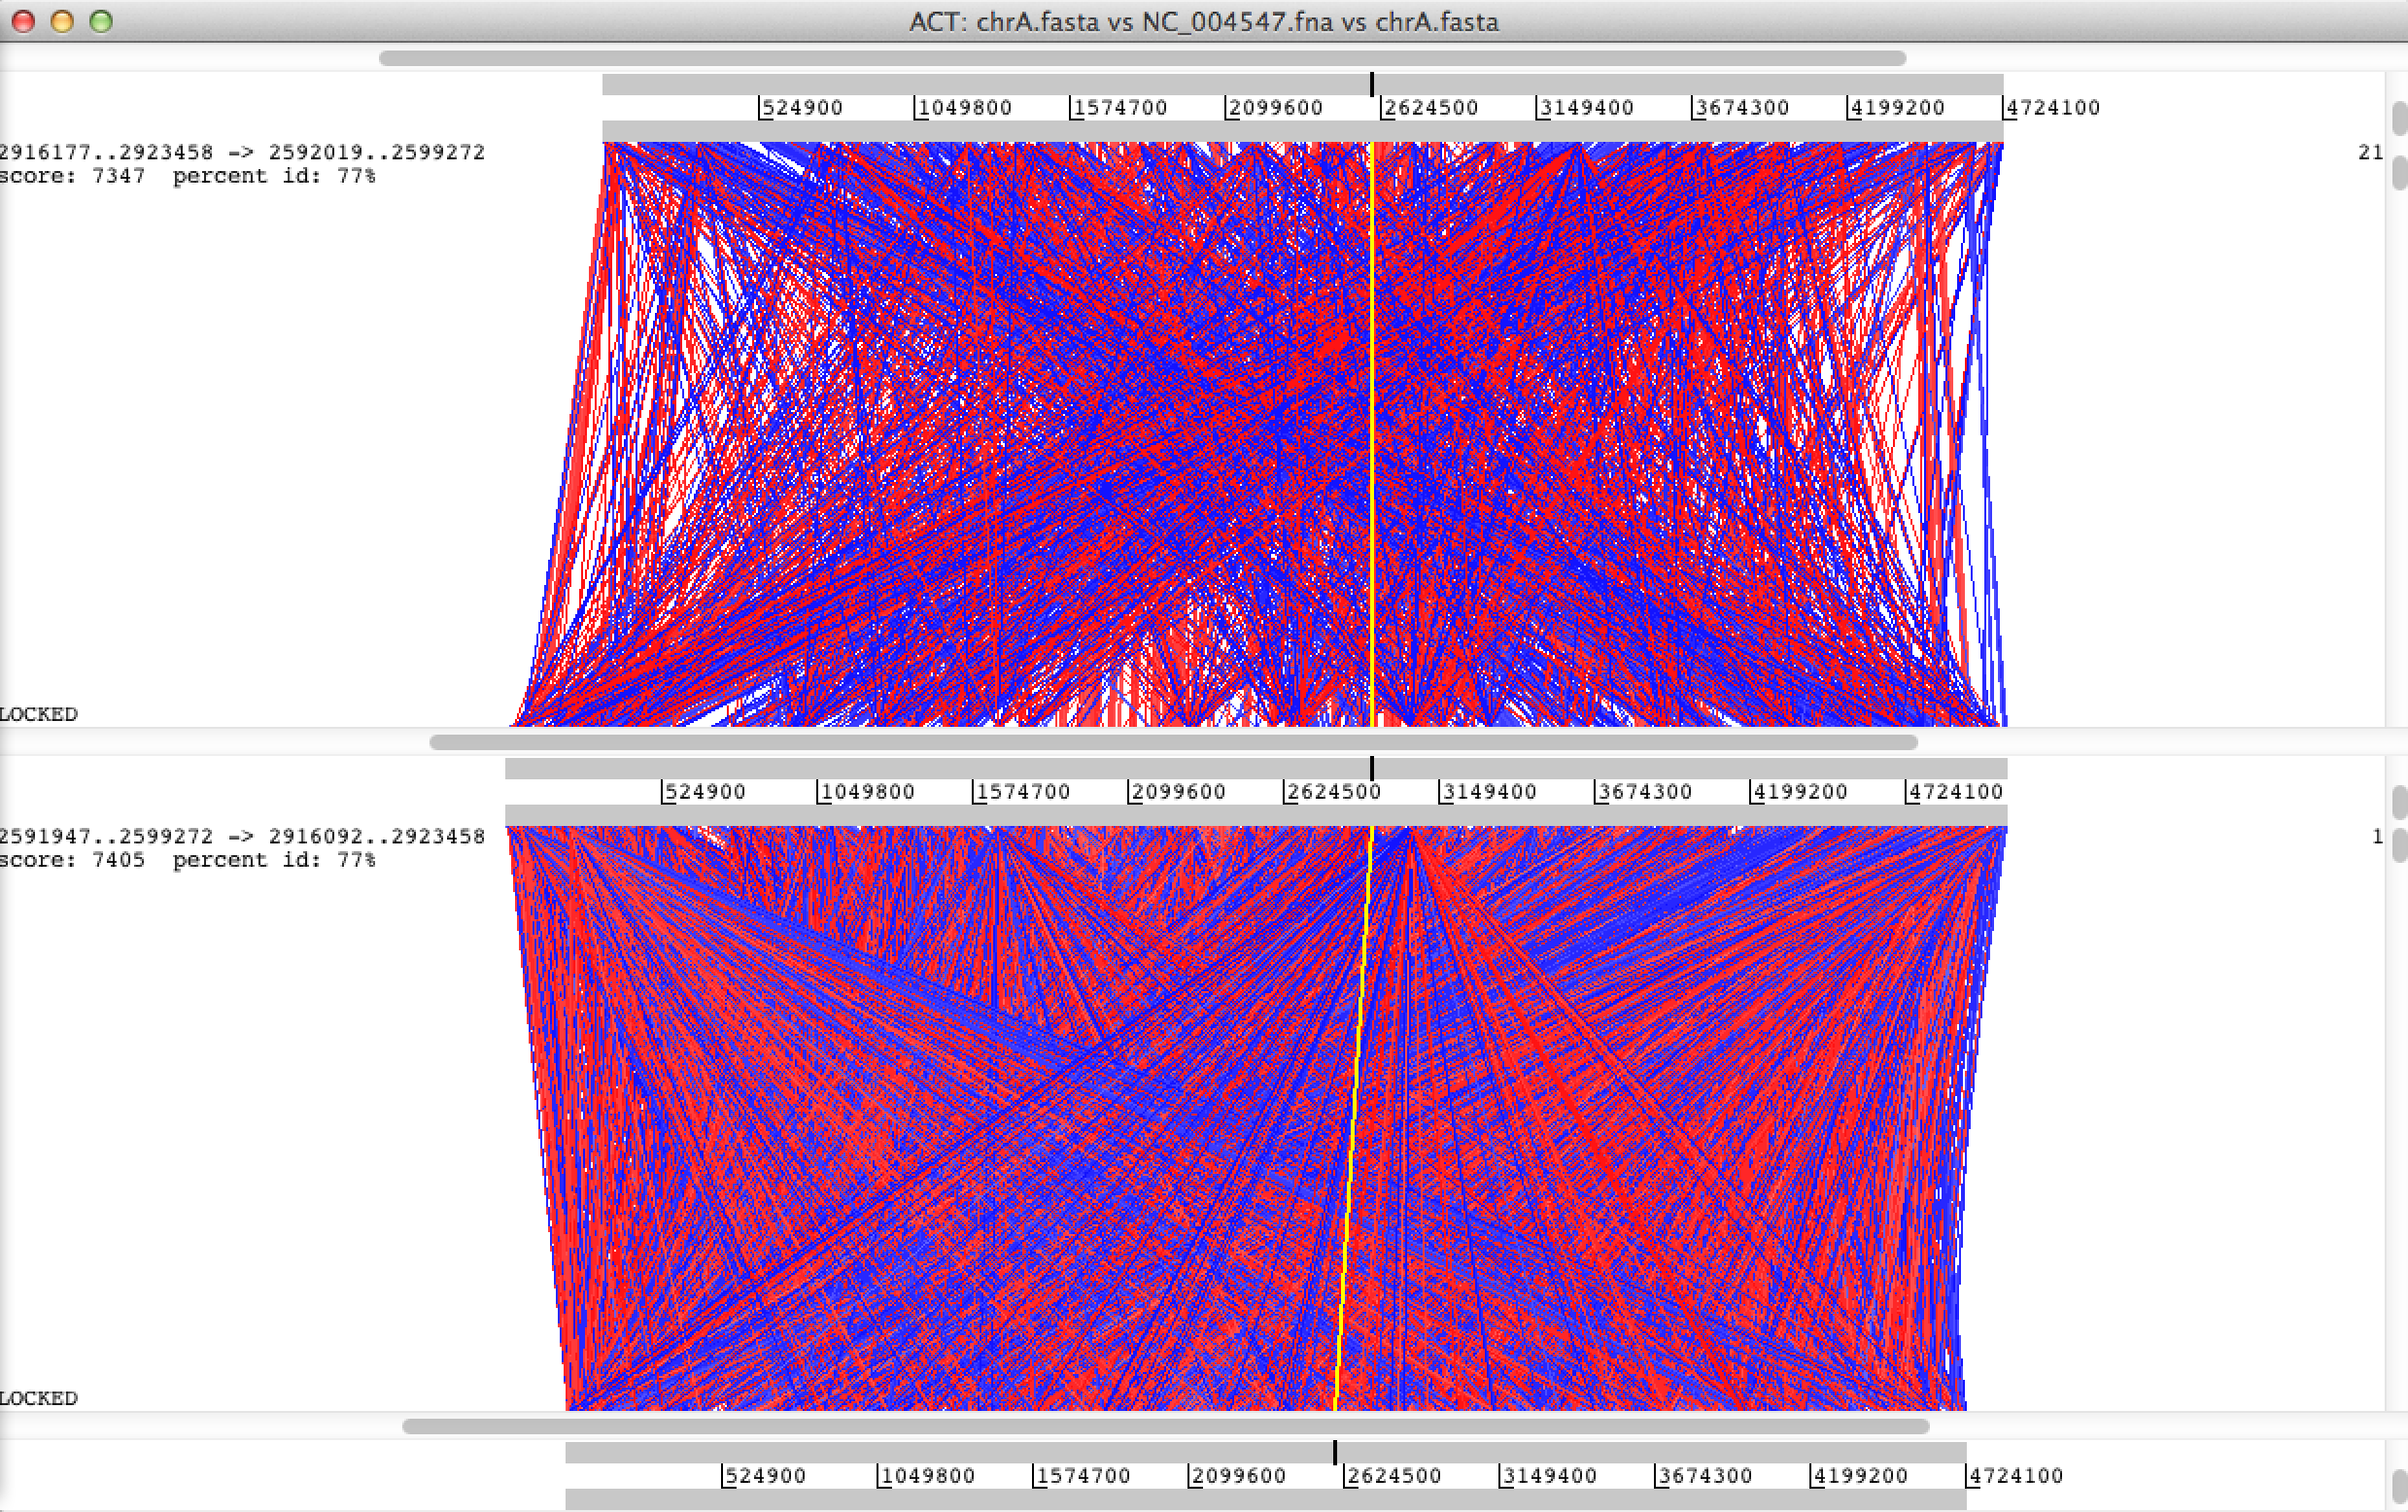
\includegraphics[width=0.8\textwidth]{images/act_wgs6}
  \end{center}
\end{frame}

\begin{frame}
  \frametitle{Remove Weak Matches}
  Use filter sliders
  \begin{center}
    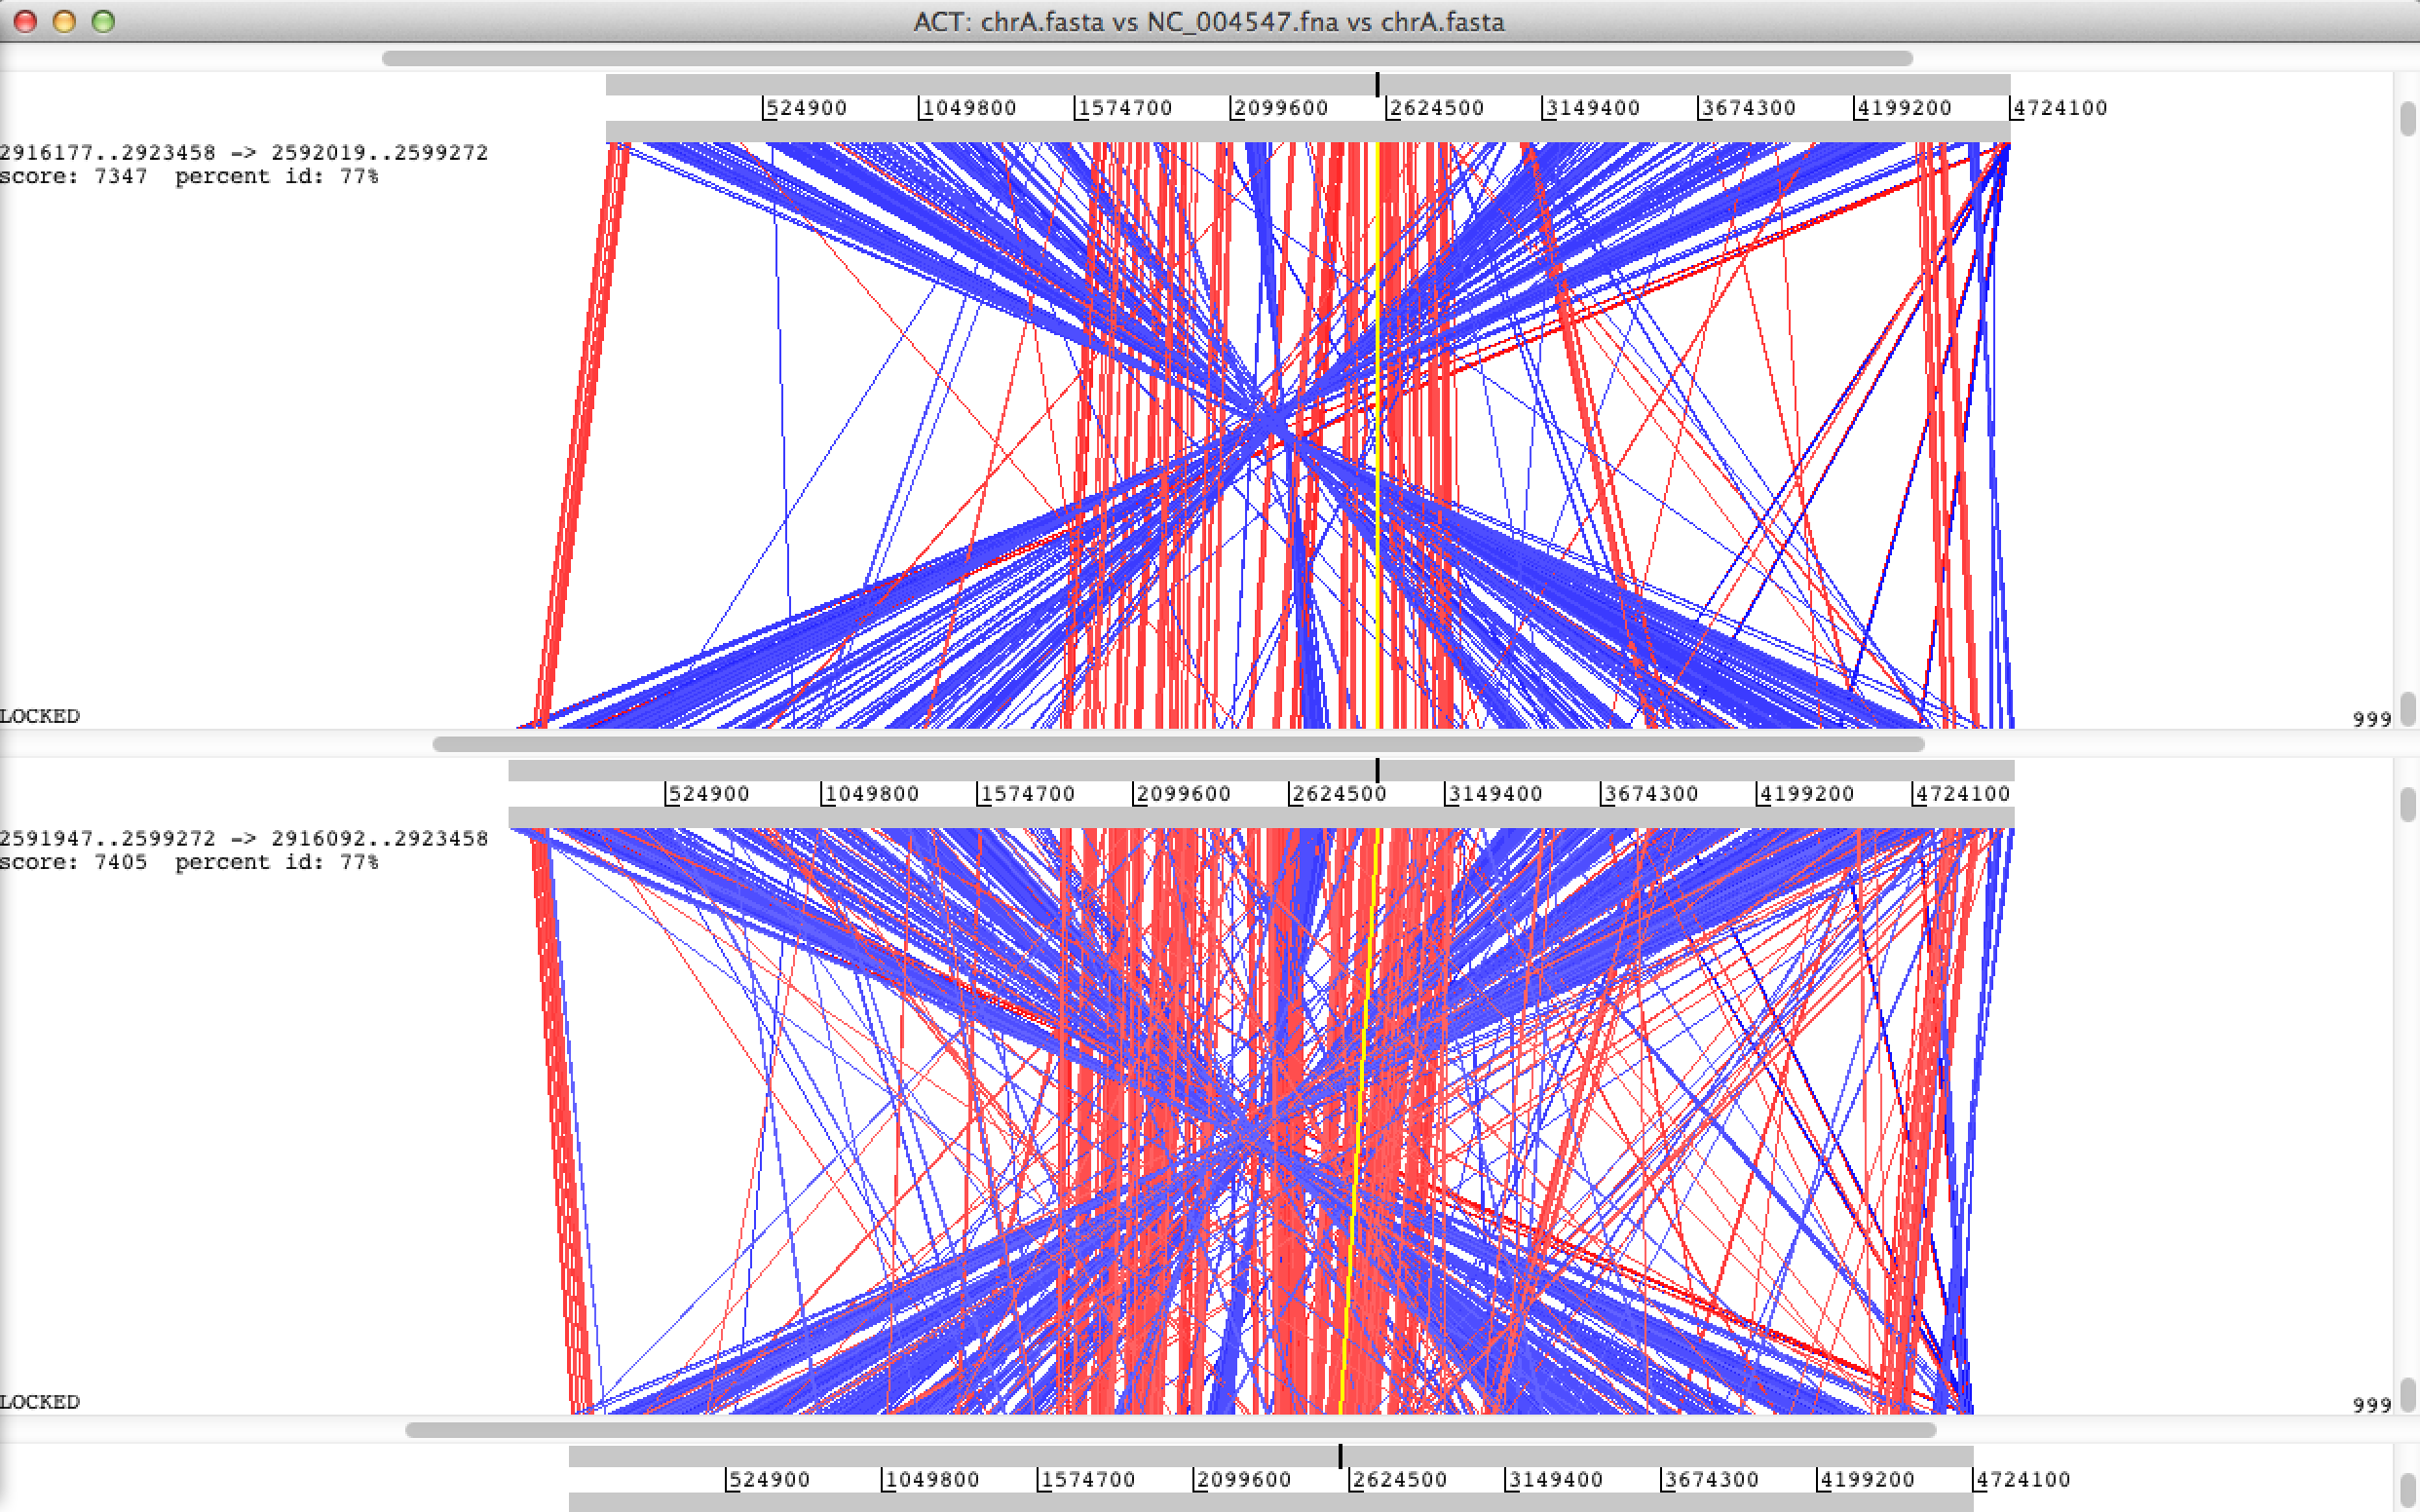
\includegraphics[width=0.8\textwidth]{images/act_wgs7}
  \end{center}
\end{frame}
